
\documentclass[11pt,a4paper]{article}
\usepackage{a4wide}\usepackage{amsmath,amssymb}
\usepackage{pdfpages}
\usepackage{dsfont}
\usepackage[latin1]{inputenc} % entree 8 bits iso-latin1
\usepackage[T1]{fontenc}      % encodage 8 bits des fontes utilisees
\usepackage[french]{babel}%typo fran�aise
\usepackage{times}
\newcommand{\R}{\mathbb{R}}\newcommand{\C}{\mathbb{C}}
\newcommand{\N}{\mathbb{N}}\newcommand{\Q}{\mathbb{Q}}

\def \I{\mathbb{I}}
\def \N{\mathbb{N}}
\def \R{\mathbb{R}}
\def \M{\mathbb{M}}
\def \Z{\mathbb{Z}}
\def \E{\mathbb{E}}
\def \F{\mathbb{F}}
\def \P{\mathbb{P}}
\def \Q{\mathbb{Q}}
\def \D{\mathbb{D}}


\def \Ac{{\cal A}}
\def \Bc{{\cal B}}
\def \Cc{{\cal C}}
\def \Dc{{\cal D}}
\def \Ec{{\cal E}}
\def \Fc{{\cal F}}
\def \Gc{{\cal G}}
\def \Hc{{\cal H}}
\def \Ic{{\cal I}}
\def \Kc{{\cal K}}
\def \Lc{{\cal L}}
\def \Pc{{\cal P}}
\def \Qc{{\cal Q}}
\def \Mc{{\cal M}}
\def \Nc{{\cal N}}
\def \Oc{{\cal O}}
\def \Sc{{\cal S}}
\def \Tc{{\cal T}}
\def \Uc{{\cal U}}
\def \Vc{{\cal V}}
\def \Wc{{\cal W}}
\def \Yc{{\cal Y}}
\def \Zc{{\cal Z}}
\def \Xc{{\cal X}}






\def \PI{\displaystyle\Pi}

\def \Sum{\displaystyle\sum}
\def \Prod{\displaystyle\prod}
\def \Int{\displaystyle\int}
\def \Frac{\displaystyle\frac}
\def \Inf{\displaystyle\inf}
\def \Sup{\displaystyle\sup}
\def \Lim{\displaystyle\lim}
\def \Liminf{\displaystyle\liminf}
\def \Limsup{\displaystyle\limsup}
\def \Max{\displaystyle\max}
\def \Min{\displaystyle\min}




\def \ni{\noindent}

\def \eps{\varepsilon}


\def \ep{\hbox{ }\hfill$\Box$}


\def\Dt#1{\Frac{\partial #1}{\partial t}}
\def\Dx#1{\Frac{\partial #1}{\partial x}}
\def\Ds#1{\Frac{\partial #1}{\partial s}}
\def\Dss#1{\Frac{\partial^2 #1}{\partial s^2}}
\def\Dy#1{\Frac{\partial #1}{\partial y}}
\def\Dyy#1{\Frac{\partial^2 #1}{\partial y^2}}
\def\Dsy#1{\Frac{\partial^2 #1}{\partial s \partial y}}
\def\Dk#1{\Frac{\partial #1}{\partial k}}
\def\Dp#1{\Frac{\partial #1}{\partial p}}
\def\Dkk#1{\Frac{\partial^2 #1}{\partial k^2}}
\def\Dpp#1{\Frac{\partial^2 #1}{\partial p^2}}
\def\Dky#1{\Frac{\partial^2 #1}{\partial k \partial y}}
\def\Dkp#1{\Frac{\partial^2 #1}{\partial k \partial p}}
\def\Dyp#1{\Frac{\partial^2 #1}{\partial y \partial p}}

\def\Dth#1{\Frac{\partial #1}{\partial \theta}}
\def\Dthi#1{\Frac{\partial #1}{\partial \theta_i}}
\def\Dthj#1{\Frac{\partial #1}{\partial \theta_j}}
\def\Dtth#1{\Frac{\partial^2 #1}{\partial \theta^2}}
\def\Dthij#1{\Frac{\partial^2 #1}{\partial \theta_i \partial \theta_j}}

\def\Dth#1{\Frac{\partial #1}{\partial \theta}}
\def\Dtth#1{\Frac{\partial^2 #1}{\partial \theta^2}}

\def\Dlam#1{\Frac{\partial #1}{\partial \lambda}}

\def\reff#1{{\rm(\ref{#1})}}

\def\beqs{\begin{eqnarray*}}
\def\enqs{\end{eqnarray*}}
\def\beq{\begin{eqnarray}}
\def\enq{\end{eqnarray}}






%%%%%\setbeamercovered{dynamic}






\newcounter{exo}
\def\cit{\addtocounter{exo}{-1}\refstepcounter{exo}\label}
\def\exo{\mbox{}\\[0em]\hspace*{0em}\bf Exercice
\addtocounter{exo}{1}\arabic{exo}.\rm\hspace{1ex}}



\begin{document}
\centerline{\sc \'Etude de Cas}  \centerline{~}
\vskip1cm \centerline{{\bf Corrig� TD 5}} \centerline{F�vrier 2011}

\exo Soit $X$ une v.a. de densit� : $$f(x) = \frac{1}{2}
e^{-|x-\theta|}, x \in  \R$$ o� $\theta$ est un param�tre r�el
inconnu.

\vspace{2mm}

\ni {\bf 1.1. Calculer $E_{\theta}[X]$ et
$\hbox{Var}_{\theta}[X]$. En d�duire un estimateur $T_n$ de
$\theta$.}

\ni Calcul de l'esp�rance :

\beqs E_{\theta}[X] &=& \frac{1}{2} \int_{-\infty}^{+ \infty} x
e^{-|x-\theta|}dx \\
&=&  \frac{1}{2} \int_{-\infty}^{+ \infty} (u + \theta) e^{-|u|}du \\
&=&  \frac{\theta}{2} \int_{-\infty}^{+ \infty}  e^{-|u|}du \\
&=& \theta \enqs

De m�me, on calcule le moment d'ordre 2 : $$E_{\theta}[X^2] = 2 +
\theta^2,$$ puis on en d�duit la variance de $X$ :
$\hbox{Var}_{\theta}(X) = 2.$

\vspace{2mm}

\ni D'apr�s la m�thode des moments, on en d�duit que la moyenne
empirique $\bar X_n$ est un estimateur de $\theta$. De plus, c'est
un estimateur convergent par la loi forte des grands nombres.

\vspace{3mm}

\ni {\bf 1.2. Construire un intervalle de confiance de niveau
asymptotique $95\%$ pour $\theta$ dans le cas o� $n = 200$.}

\vspace{2mm}

D'apr�s le Th�or�me Central Limite, on obtient:

$$ \sqrt{n} \left(\frac{\bar X_n - E_{\theta}[X] }{\sqrt{Var_{\theta}(X)}}
\right)\: \Rightarrow^{\hbox{loi}} \: \Nc (0, 1).$$

on obtient l'intervalle de confiance asymptotique suivant :

$$
\hbox{IC}(\theta) = \left[\bar X_n - u_{\frac{\alpha}{2}}
\sqrt{\frac{2}{n}}\;,\; \bar X_n + u_{\frac{\alpha}{2}}
\sqrt{\frac{2}{n}}\right]$$


\exo  On rappelle que dans le mod�le uniforme $\Pc = \{\Uc [0,
\theta], \theta >0 \}$, l'Estimateur du Maximum de Vraisemblance
de $\theta$ est $\hat \theta_n = \max(X_1,...,X_n).$

\vspace{2mm}

\ni {\bf 2.1. Pour $x \in \R$, calculer $\P_{\theta}(\frac{\hat
\theta_n}{\theta} \leq x)$ et en d�duire que la loi de $\frac{\hat
\theta_n}{\theta}$ ne d�pend pas de $\theta$.}

\vspace{2mm}

On a d�j� vu en cours que $X_{(n)}$ admet comme densit� $y \mapsto
\frac{n}{\theta^n} y^{n-1} {\bf 1}_{[0, \theta]}(y)$. Comme
$\theta$ est un param�tre d'�chelle, $\frac{X_{(n)}}{\theta}$ a
pour densit� $z \mapsto n z^{n-1} {\bf 1}_{[0, 1]}(z)$.

\vspace{2mm}

Donc $\frac{\theta}{X_{(n)}}$ a pour densit� $f: t \mapsto
\frac{n}{t^{n+1}}{\bf 1}_{[1, \infty]}(t)$. Ainsi,
$\frac{\theta}{X_{(n)}}$ est bien une statistique libre pour
$\theta$. Sa densit� est bien unimodale puisque constante (et
�gale � $0$ avant $1$ et strictement d�croissant apr�s $1$. La
valeur $1$ est l'unique mode et point de discontinuit�.

\vspace{2mm}

\ni {\bf 2.2. Construire un intervalle de confiance de niveau $1 -
\alpha$ pour $\theta$.}

\vspace{2mm}

On cherche le plus court intervalle $[a,b]$ tel que
$$P(a \leq \frac{\theta}{X_{(n)}} \leq b) = \int_a^b f(t) dt = 1 -
\alpha$$

Comme $f$ est une fonction strictement d�croissante sur $]1,
\infty[$, n�cessairement $a= 1$, alors

$$\int_1^b \frac{n}{t^{n+1}} dt = 1 - \alpha$$
soit $$b= \alpha^{-1/n}$$

$P(1 \leq \frac{\theta}{X_{(n)}} \leq \alpha^{-1/n}) = 1 - \alpha$
s'�crit $$P(X_{(n)} \leq \theta \leq \alpha^{-1/n} X_{(n)}) = 1 -
\alpha$$ autrement, l'IC s'�crit
$$IC = ]X_{(n)} \:;\: \alpha^{-1/n} X_{(n)}[$$

\vspace{2mm}

\exo {\bf 3.1.} La vraisemblance associ�e � l'�chantillon est
d�finie par:

\vspace{2mm}

$$ L(x,\theta) \;=\; \exp \left(- \Sum_{i=1}^n (x_i - \theta)
\right) \Pi_{i=1}^n{\bf 1}_{[\theta, \infty[}(x_i)$$

\ni {\bf 3.2.} $L(x,\theta)$ est maximum en $\theta$ ssi
$\Pi_{i=1}^n {\bf 1}_{[\theta, \infty[}(x_i) = 1$. Autrement dit,

\vspace{2mm}

$\forall i=1,...,n, \; \theta \leq x_i$, donc $\Inf_{1\leq i \leq
n} x_i \geq \theta$. D'o� $\hat \theta_n = \Inf_{1\leq i \leq n}
X_i$ est l'EMV.

\vspace{2mm}

\ni {\bf 3.3.} La loi densit� de la loi de $\hat \theta_n$ est
d�finie par:

$$f_{\hat \theta_n}(x,\theta) = n e^{-n(x-\theta)} {\bf 1}_{[\theta,
\infty[}(x)$$

D'o�  $E[\hat \theta_n] = \theta - \frac{1}{n}$.

\vspace{2mm}

\ni {\bf 3.4.} $T_n = \hat \theta_n - \theta$ est de loi densit�:

$$f_{T_n}(x,\theta) = n e^{-nx} {\bf 1}_{[0,
\infty[}(x)$$

C'est donc une statistique libre pour $\theta$.

\vspace{2mm}

\ni {\bf 3.5.} Pour un $\alpha$ donn�, on cherche un $A = A(\hat
\theta_n)$ tel que $P(A \leq \theta \leq \hat \theta_n) = 1 -
\alpha$. On a :

$$P(A \leq \theta \leq \hat \theta_n) = P(0 \leq T_n \leq \hat \theta_n - A) =
 F_{T_n}(\hat \theta_n - A) = 1 - \alpha$$

 Soit $A= \hat \theta_n -  F_{T_n}^{-1}(1 - \alpha)$ soit $A= \hat \theta_n +  \frac{1}{n} \log
 \alpha$.

\vspace{2mm}

L'intervalle de confiance est :

$$\left[ \hat \theta_n +  \frac{1}{n} \log
 \alpha)   \;;\;\hat \theta_n\right]$$

\ni {\bf 3.6. et 3.7.} A faire vous m�me!


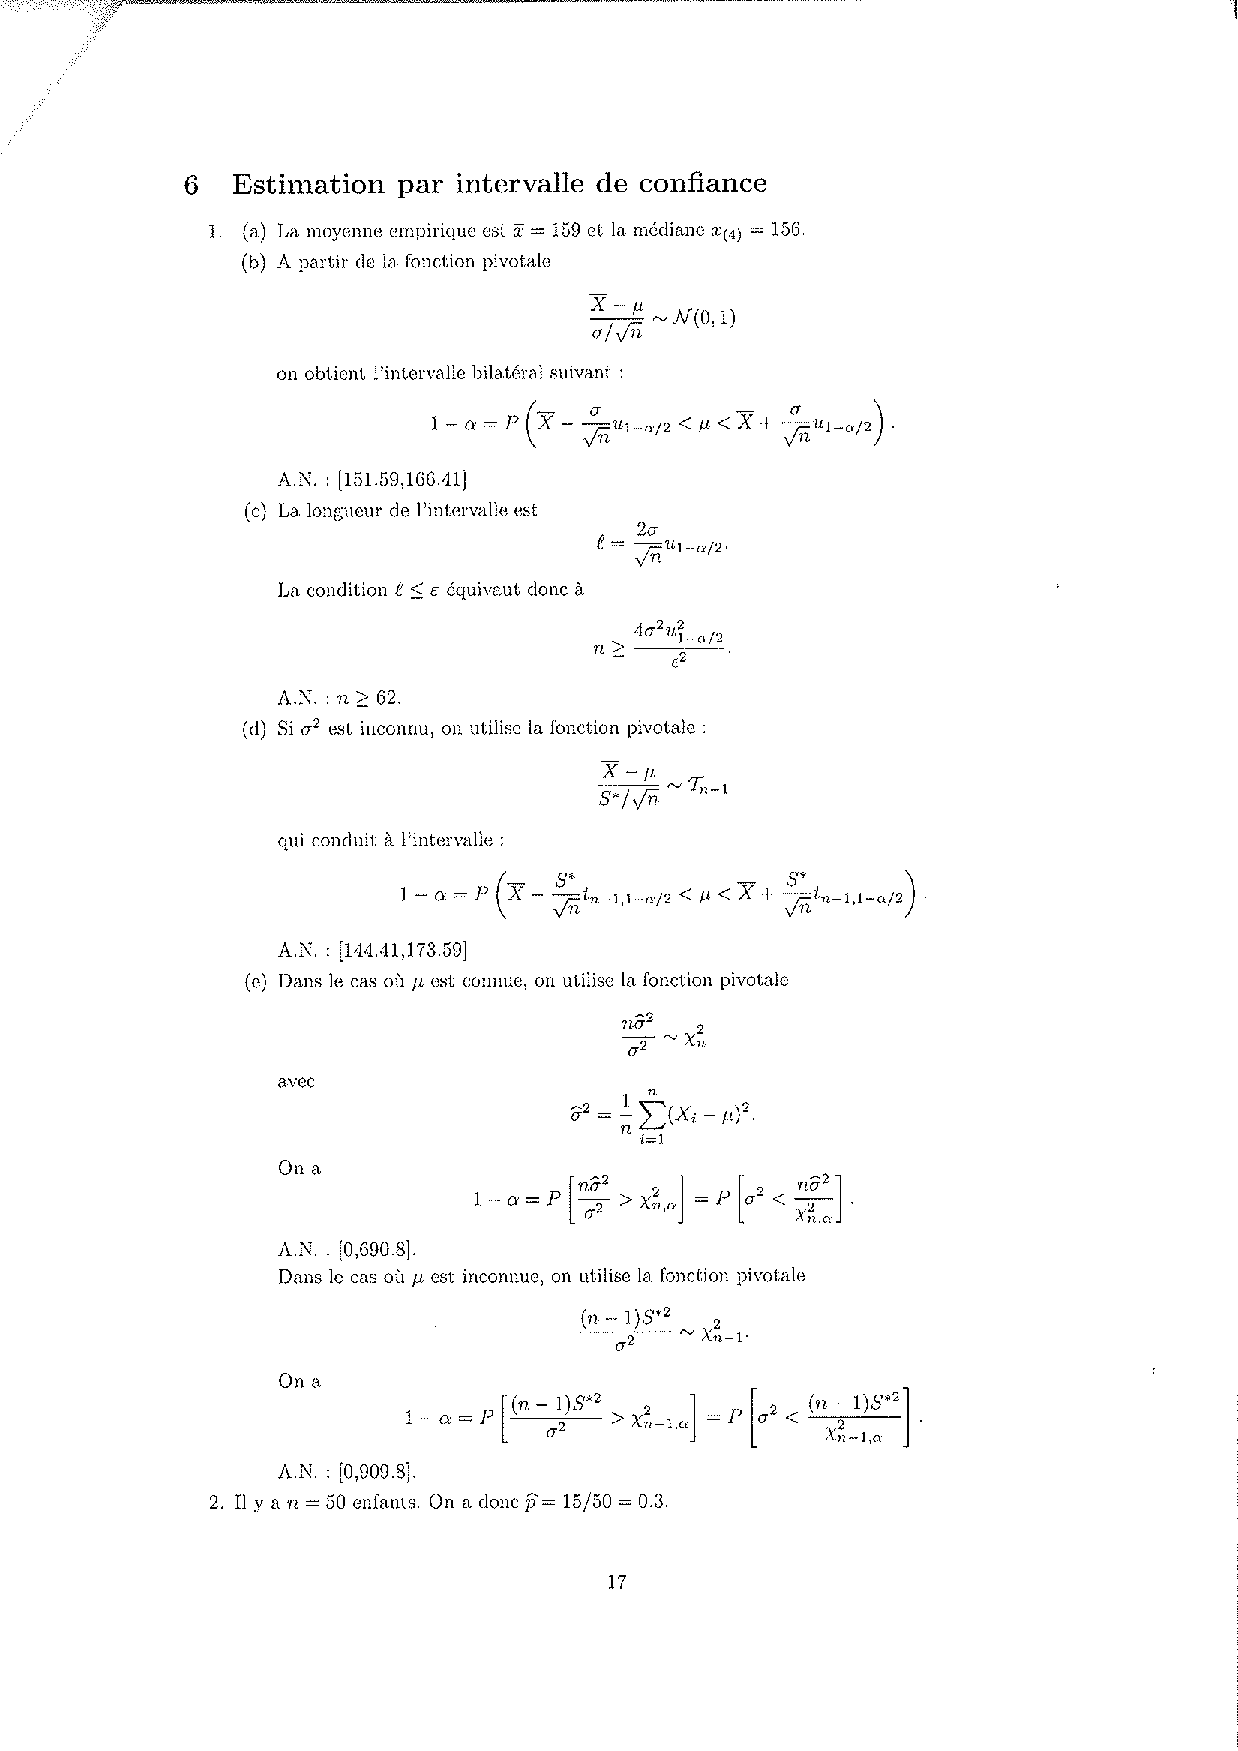
\includepdf{0911_001.pdf}

\end{document}
